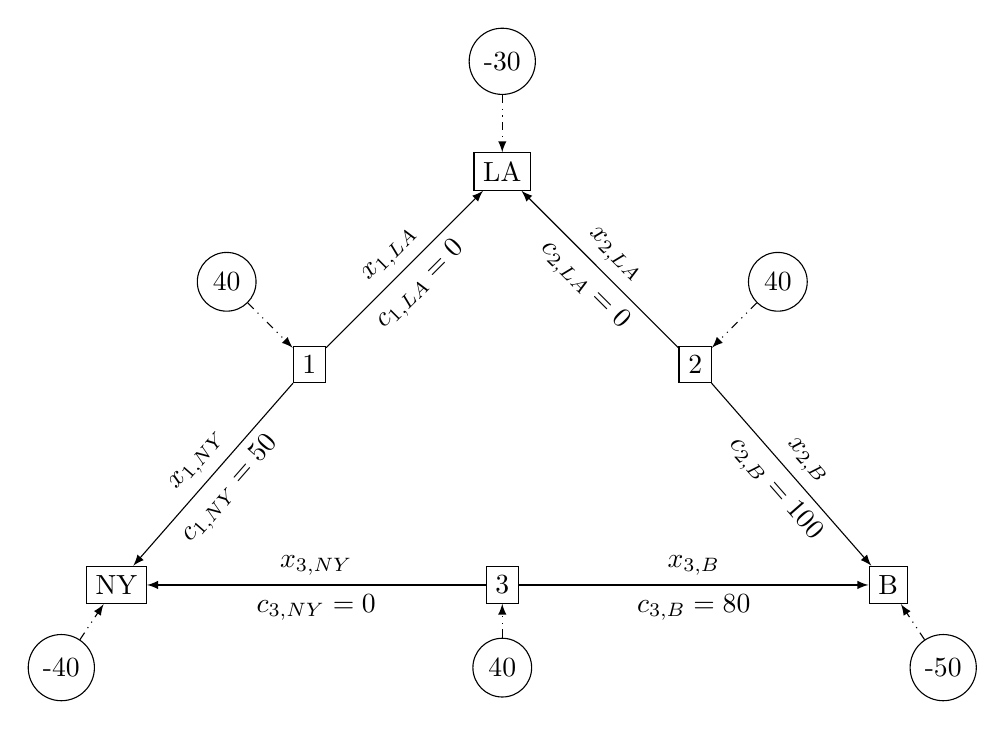
\begin{tikzpicture}[scale=0.7]
 \draw node[rectangle, draw] (LA) at (0,7) {LA};
 \draw node[rectangle, draw] (NY) at (-7,-0.5) {NY};
 \draw node[rectangle, draw] (B) at (7,-0.5) {B};
 \draw node[rectangle, draw] (1) at (-3.5,3.5) {1};
 \draw node[rectangle, draw] (2) at (3.5,3.5) {2};
 \draw node[rectangle, draw] (3) at (0,-0.5) {3};

 \draw[-latex] (2) -- (LA)
 node[midway, sloped, above] {$x_{2, LA}$}
 node[midway, sloped, below] {$c_{2, LA}=0$};

 \draw[-latex] (2) -- (B)
 node[midway, sloped, above] {$x_{2, B}$}
 node[midway, sloped, below] {$c_{2, B}=100$};

 \draw[-latex] (1) -- (LA)
 node[midway, sloped, above] {$x_{1, LA}$}
 node[midway, sloped, below] {$c_{1, LA}=0$};

 \draw[-latex] (1) -- (NY)
 node[midway, sloped, above] {$x_{1, NY}$}
 node[midway, sloped, below] {$c_{1, NY}=50$};

 \draw[-latex] (3) -- (B)
 node[midway, sloped, above] {$x_{3, B}$}
 node[midway, sloped, below] {$c_{3, B}=80$};

 \draw[-latex] (3) -- (NY)
 node[midway, sloped, above] {$x_{3, NY}$}
 node[midway, sloped, below] {$c_{3, NY}=0$};

 \draw node[circle, draw] (4) at (0, 9) {-30};
 \draw[-latex, dashdotdotted] (4)--(LA);
 \draw node[circle, draw] (5) at (-5, 5) {40};
 \draw[-latex, dashdotdotted] (5)--(1);
 \draw node[circle, draw] (6) at (5, 5) {40};
 \draw[-latex, dashdotdotted] (6)--(2);
 \draw node[circle, draw] (7) at (-8, -2) {-40};
 \draw[-latex, dashdotdotted] (7)--(NY);
 \draw node[circle, draw] (8) at (8, -2) {-50};
 \draw[-latex, dashdotdotted] (8)--(B);
 \draw node[circle, draw] (9) at (0, -2) {40};
 \draw[-latex, dashdotdotted] (9)--(3);
\end{tikzpicture}

